\chapter{Theoretical basis}

\section{Face detection}
A way to approach the face detection problem is to see it as an instance of the more general problem of object detection. With this in mind, the Dalal-Triggas detector \cite{DalalTriggs05}, which won the 2006 PASCAL object detection challenge, uses a single filter of Histogram of Oriented Gradients (HOG) as features to represent the objects of a class. The detector consists of sliding a window over the image at different scales, computing the HOG for each position and then using a classifier to determine whether the content of the window belonged to a class.
\begin{figure}[h]
	\begin{center}
		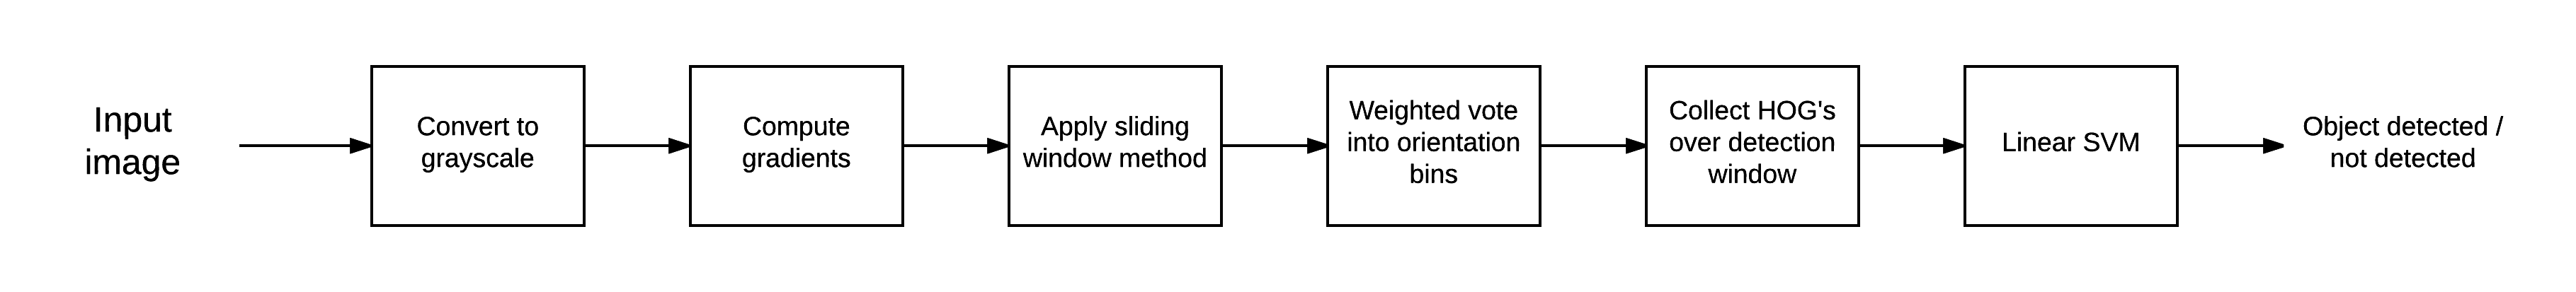
\includegraphics[width=15cm]{Process_of_detecting_an_object_with_HOG}
		\caption[Process flow of detecting an object in an image]{The step-by-step process of detecting an object in an image generalized from the person detection method presented in \cite{DalalTriggs05}}
	\end{center}
\end{figure}
The process of computing the HOG descriptor for a window, as described in \cite{DalalTriggs05}, respects the following steps: 

We convert the image from RGB space to grayscale applying for each pixel the following formula: 
\begin{align}
	I(x,y) = 0.2989 * R(x,y) + 0.5870 * G(x,y) + 0.1140 * B(x,y)
	\label{formula:intensity_function}
\end{align}
where $I$ is the intensity function in the gray image and R, G and B are the values of the red, green, respectively blue channel of the RGB image. This way we are normalizing the colors.
	 
We slide a detection window of size $64\times128$ over the gray image with a step of 32 pixels. For each position, we divide the window in four $16\times16$ pixel blocks of four $8\times8$ pixel cells. For each pixel cell, we compute a histogram of 9 orientation bins in $0^{\degree}-180{\degree}$ (unsigned gradient) range from the gradients of each pixel. This can be seen as a voting scheme, where each pixel contributes to a single orientation bin. As noted in \cite{DalalTriggs05} increasing the number of bins beyond 9 brings little accuracy improvement and allowing signed orientation bins in the range $0^{\degree}-360^{\degree}$ decreases the performance.

We define the gradient orientation $\theta$ for each pixel as:
\begin{align}
	\theta = tan^{-1}\frac{g_{y}}{g_{x}}
\end{align}
where $g_{x}$ and $g_{y}$ are the derivatives with respect to the $x\ axis$, respectively $y\ axis$ of the $I$ intensity function described in Formula \ref{formula:intensity_function}. $I$ being a discrete function, we can approximate the derivative with the convolution of $I$ and a kernel $g$. Letting $g$ be a 1D filter of size $m$ we define the convolution operation with respect to the x axis as:
\begin{align}
	(I*g)(x,y) = \sum_{j=1}^{m}g(j)\cdot I(x-j+m/2, y)
\end{align}
and with respect to the y axis we define it as:
\begin{align}
	(I*g)(x,y) = \sum_{j=1}^{m}g(j)\cdot I(x,y-j+m/2)
\end{align}
But $g$ can take the form several filters as: 1-D point derivative: uncentered, centered, cubic corrected as can be seen in Formula \ref{formula:1d_point_derivative}
\begin{align}
(\begin{smallmatrix}
-1 & +1
\end{smallmatrix}), 
(
\begin{smallmatrix}
-1 & 0 & +1
\end{smallmatrix}), 
 ( 
 \begin{smallmatrix}
 -1 & -8 & 0 & +8 & +1
 \end{smallmatrix})
 \label{formula:1d_point_derivative}
\end{align}
$3\times3$ Sobel mask (Formula \ref{formula:sobel_mask_derivative})
\begin{align}
\bigl(
\begin{smallmatrix}
+1 & 0 & -1 \\
+2 & 0 & -2 \\
+1 & 0 & -1 \\
\end{smallmatrix}
\bigr)
\label{formula:sobel_mask_derivative}
\end{align}
or 2-D diagonal ones (Formula \ref{formula:2d_point_derivative})
\begin{align}
(
\begin{smallmatrix}
	 0 & 1\\
    -1 & 0
\end{smallmatrix}
),
(
\begin{smallmatrix}
	-1 & 0\\
	 0 & -1
\end{smallmatrix}
)
\label{formula:2d_point_derivative}
\end{align}
As concluded in \cite{DalalTriggs05} simple, 1-dimensional masks work best. We concatenate the histograms computed for each $8\times8$ pixel cells resulting in a vector of 36 features. Lastly, for the entire window containing four $16\times16$ pixel blocks results, by concatenation, a feature vector of 144 dimensions.
We then use this descriptor to determine whether in the current window appears an instance of an object that we are looking for.
